% !TEX root =  ../FinalReport.tex

\newcommand{\npoisson}{N_{Poisson}}

\chapter{Results}\label{sec:Results}
% Some of the tests for non-functional requirements required more in-depth exploration and results gathering.
% This section shows the data gathered to evaluate these requirements.
Some non-functional requirements are based on comparisons to the original program or on tests that require more detailed analysis.
This section shows the data used to evaluate these more complex requirements.
The speed of the simulation is compared the original, and the performance scaling with simulation grid size is measured and justified.
Simulation accuracy vs. the original is evaluated.
GPU Utilization of both the simulation and visualization is measured, and shown to be as high as possible given the design.
Multiple programs are used to try and find memory leaks, and show the program is leak-free.
These results are then used in the Evaluation (\cref{sec:Evaluation}).

\pagebreak
\section{Simulation}
\todomark{Not sure what to put here}

\subsection{Speed}\label{sec:Results:Sim:Speed}

% \begin{figure}
%     \centering
%     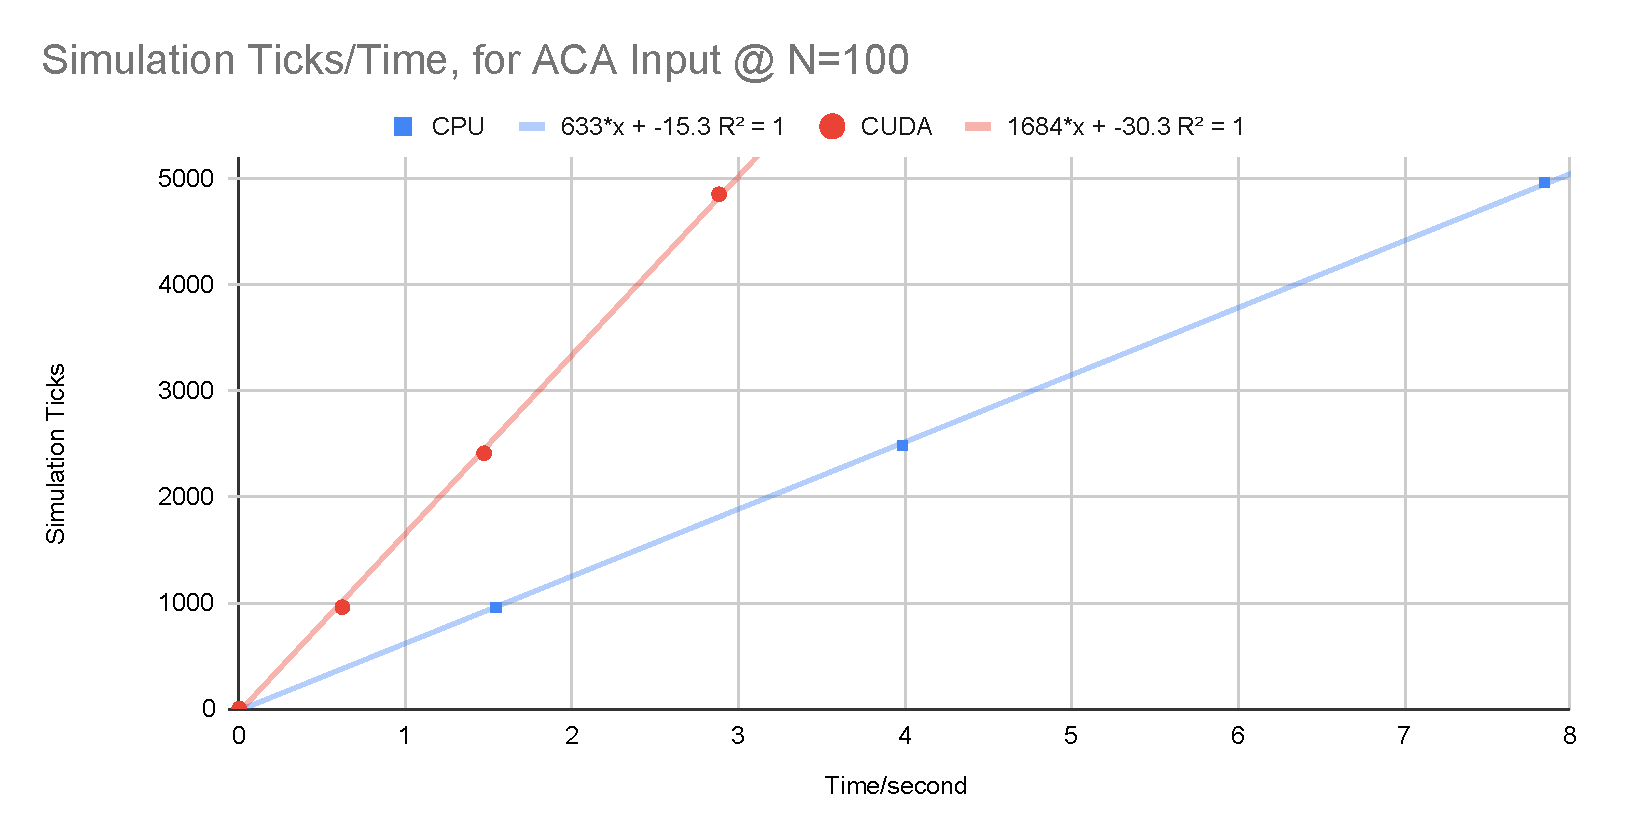
\includegraphics[width=\linewidth]{Ch62Results/figures/temp_ticks_vs_time_aca.pdf}
%     \caption{Ticks executed over time}
%     \label{fig:results:ticks_vs_time}
% \end{figure}

\begin{figure}
    \centering
    \resizebox{\linewidth}{!}{%
    \begin{tikzpicture}
    \begin{axis}[
        title={Ticks Executed over Time},
        ylabel={Ticks Executed},
        xlabel={Time (\si{\second})},
        width=\linewidth,
        height=15em,
    ]
    \addplot table [x=Time, y=ticks_cpu, col sep=space, ignore chars={\,}] {Ch62Results/figures/data/time_ticks_cpu.csv};
    \addlegendentry{CPU};
    
    \addplot table [x=Time, y=ticks_cuda, col sep=space, ignore chars={\,}] {Ch62Results/figures/data/time_ticks_cuda.csv};
    \addlegendentry{CUDA};

    \end{axis}
    \end{tikzpicture}
    }
    
    \caption{Ticks executed over time}
    \label{fig:results:ticks_vs_time}
\end{figure}

Each tick of a simulation performs the same amount of work, so it was hypothesized that the number of ticks per second would be a suitable metric for measuring simulation speed.
To verify this, the initial ACA input was simulated with the CUDA and CPU backends for 10, 25, and 50 simulation-seconds with $\npoisson = 100$.
As shown in \cref{fig:results:ticks_vs_time}, elapsed real-time is directly proportional to number of ticks executed with R-values of $R^2_{CPU} = 0.9999$ and $R^2_{CUDA} = 0.9996$.
This proves that ticks-per-second can be used to accurately compare CUDA/CPU performance.

% \begin{figure}
%     \centering
%     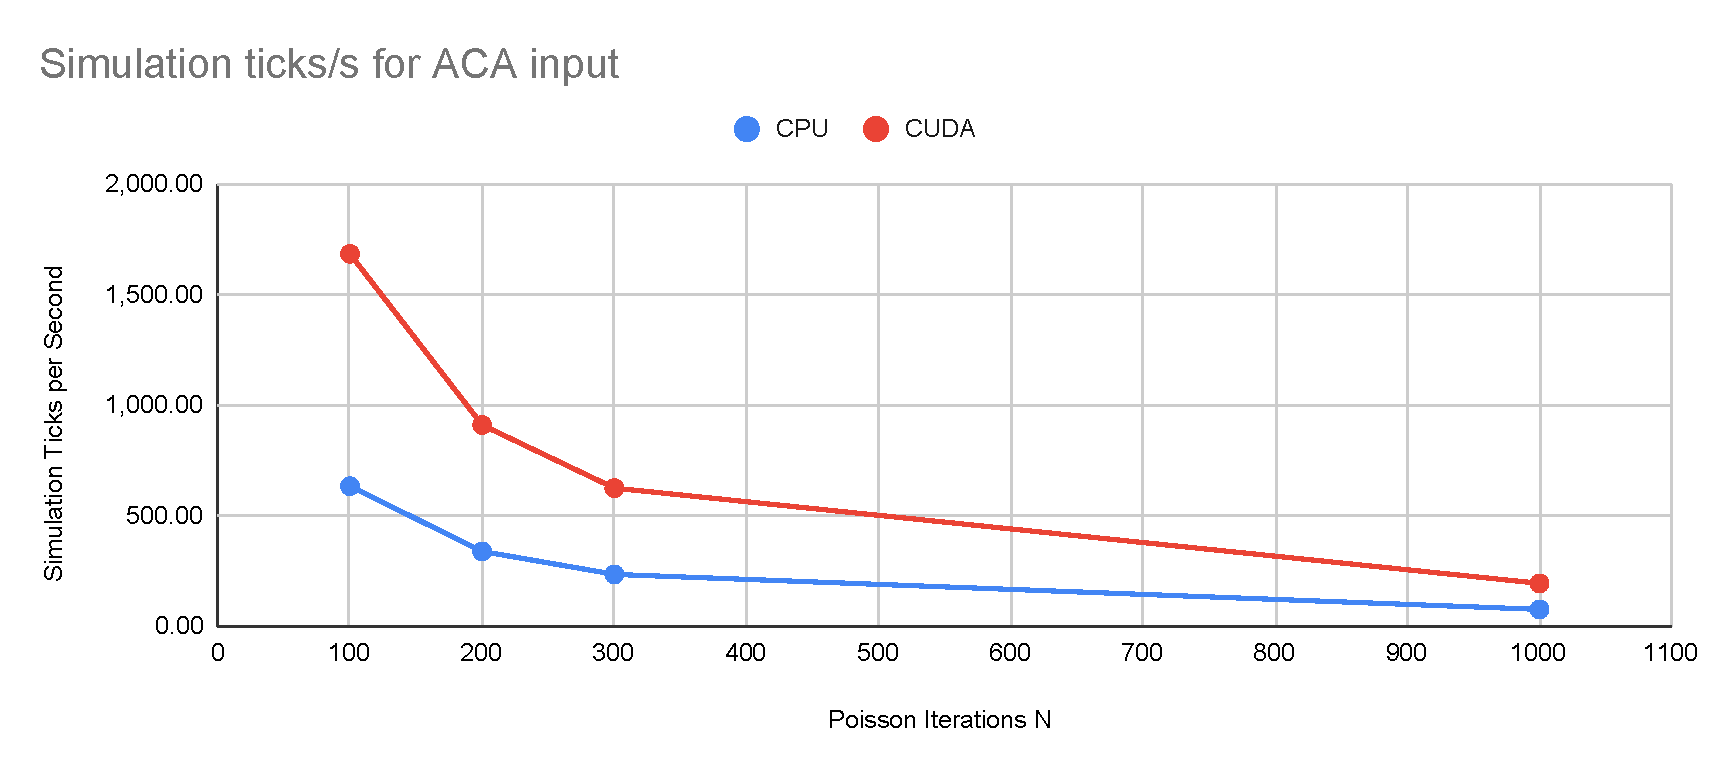
\includegraphics[width=\linewidth]{Ch62Results/figures/temp_ticks_per_second_vs_iters_aca.pdf}
%     \caption{Simulation Tick Speed vs. Poisson Iterations}
%     \label{fig:results:ticks_per_second_bar_aca}
% \end{figure}

\begin{figure}
    \centering
    \begin{tikzpicture}
    \begin{axis}[
        % title={Simulation Tick Speed},
        ylabel={Tick Rate (\si{\per\second})},
        xlabel={Poisson Iterations N},
        % xtick = {100, 200, 300, 400},
        xtick=data,
        symbolic x coords={100, 200, 300, 1000},
        width=\linewidth,
        height=15em,
        bar width=30pt,
        x tick style = transparent,
        ybar,
        enlarge x limits=0.25,
        ymin=0
    ]
    \addplot[ fill=blue] table [x=iters, y=cuda_speed, col sep=semicolon, ignore chars={\,}] {Ch62Results/figures/data/ticks_per_second.csv};
    \addlegendentry{CUDA};
    \addplot[ fill=red] table [x=iters, y=cpu_speed, col sep=semicolon, ignore chars={\,}] {Ch62Results/figures/data/ticks_per_second.csv};
    \addlegendentry{CPU};
    
    % \addplot[mark=none, black] {1.0};
    \end{axis}
    \end{tikzpicture}
    \caption{Simulation Tick Speed vs. Poisson Iterations}
    \label{fig:results:ticks_per_second_bar_aca}
\end{figure}


% \begin{figure}
%     \centering
%     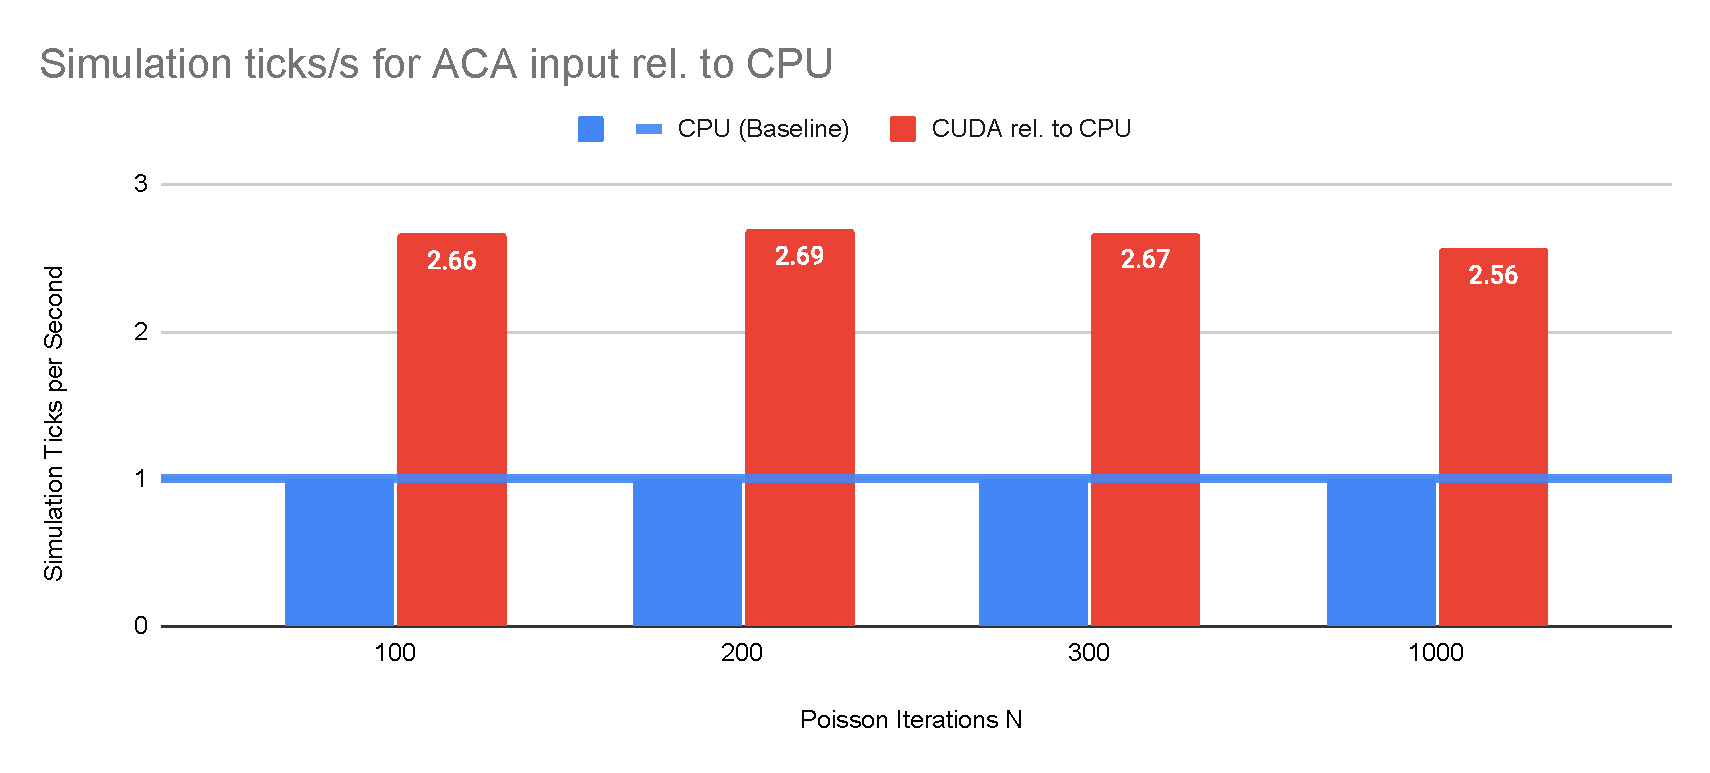
\includegraphics[width=\linewidth]{Ch62Results/figures/temp_ticks_per_second_vs_iters_rel_cpu_aca.pdf}
%     \caption{Simulation Tick Speed relative to CPU}
%     \label{fig:results:ticks_per_second_bar_rel_cpu_aca}
% \end{figure}

\begin{figure}
    \centering
    \begin{tikzpicture}
    \begin{axis}[
        % title={Simulation Tick Speed},
        ylabel={Tick Rate (\si{\per\second})},
        xlabel={Poisson Iterations N},
        % xtick = {100, 200, 300, 400},
        xtick=data,
        symbolic x coords={100, 200, 300, 1000},
        width=\linewidth,
        height=20em,
        bar width=30pt,
        x tick style = transparent,
        ybar,
        enlarge x limits=0.25,
        ymin=0, ymax=3
    ]
    
    \addplot[ fill=blue] table [x=iters, y=cpu_speed_rel, col sep=semicolon, ignore chars={\,}] {Ch62Results/figures/data/ticks_per_second.csv};
    \addlegendentry{CPU};
    
    \addplot[ fill=red] table [x=iters, y=cuda_speed_rel, col sep=semicolon, ignore chars={\,}] {Ch62Results/figures/data/ticks_per_second.csv};
    \addlegendentry{CUDA};

    
    \draw [black, style={line width=2pt}] ({rel axis cs:0,0}|-{axis cs:100,1.0}) -- ({rel axis cs:1,0}|-{axis cs:100,1.0});% node [pos=0.33, above] {KPI};
    
    \end{axis}
    \end{tikzpicture}
    \caption{Simulation Tick Speed relative to CPU}
    \label{fig:results:ticks_per_second_bar_rel_cpu_aca}
\end{figure}

The ticks-per-second for CPU and CUDA are shown in \cref{fig:results:ticks_per_second_bar_aca}, varying $\npoisson \in {100, 200, 300, 1000}$.
As expected the ticks-per-second decreases as more iterations are added, and CUDA is consistently faster than the CPU.
When normalized relative to the CPU speed (\cref{fig:results:ticks_per_second_bar_rel_cpu_aca}), CUDA is shown to consistently have \~2.6x the ticks-per-second of the CPU, i.e. CUDA is consistently 2.6x faster than the CPU. 
The Poisson stage is likely less sped up than the others, as the speedup for $\npoisson{} = 1000$ (where the Poisson stage dominates) is less than that for lower $\npoisson{}$ values.

\subsubsection{Scaling}
To determine how the implementations scale with grid resolution, a simple simulation with no obstacle squares was performed for resolutions between 260~x~130 and 4096~x~2048.
As the amount of work per simulation tick varies with grid size, each tick is multiplied by the number of grid cells and number of Poisson iterations to determine the number of operations (\si{op}s) executed, and  mega-operations-per-second (\si{\mega\op\per\second}) is used to measure performance.
The increasing size is measured in the total amount of memory (in \si{\mega\byte}) required for a full Poisson red/black iteration, equal to three full size matrices: the pressure matrix, the $\beta$ matrix, and the $rhs$ matrix.
\cref{fig:results:throughput_over_size} shows \si{\mega\op\per\second} for CUDA and CPU against the memory required in \si{\mega\byte}.

\begin{figure}
    \centering
    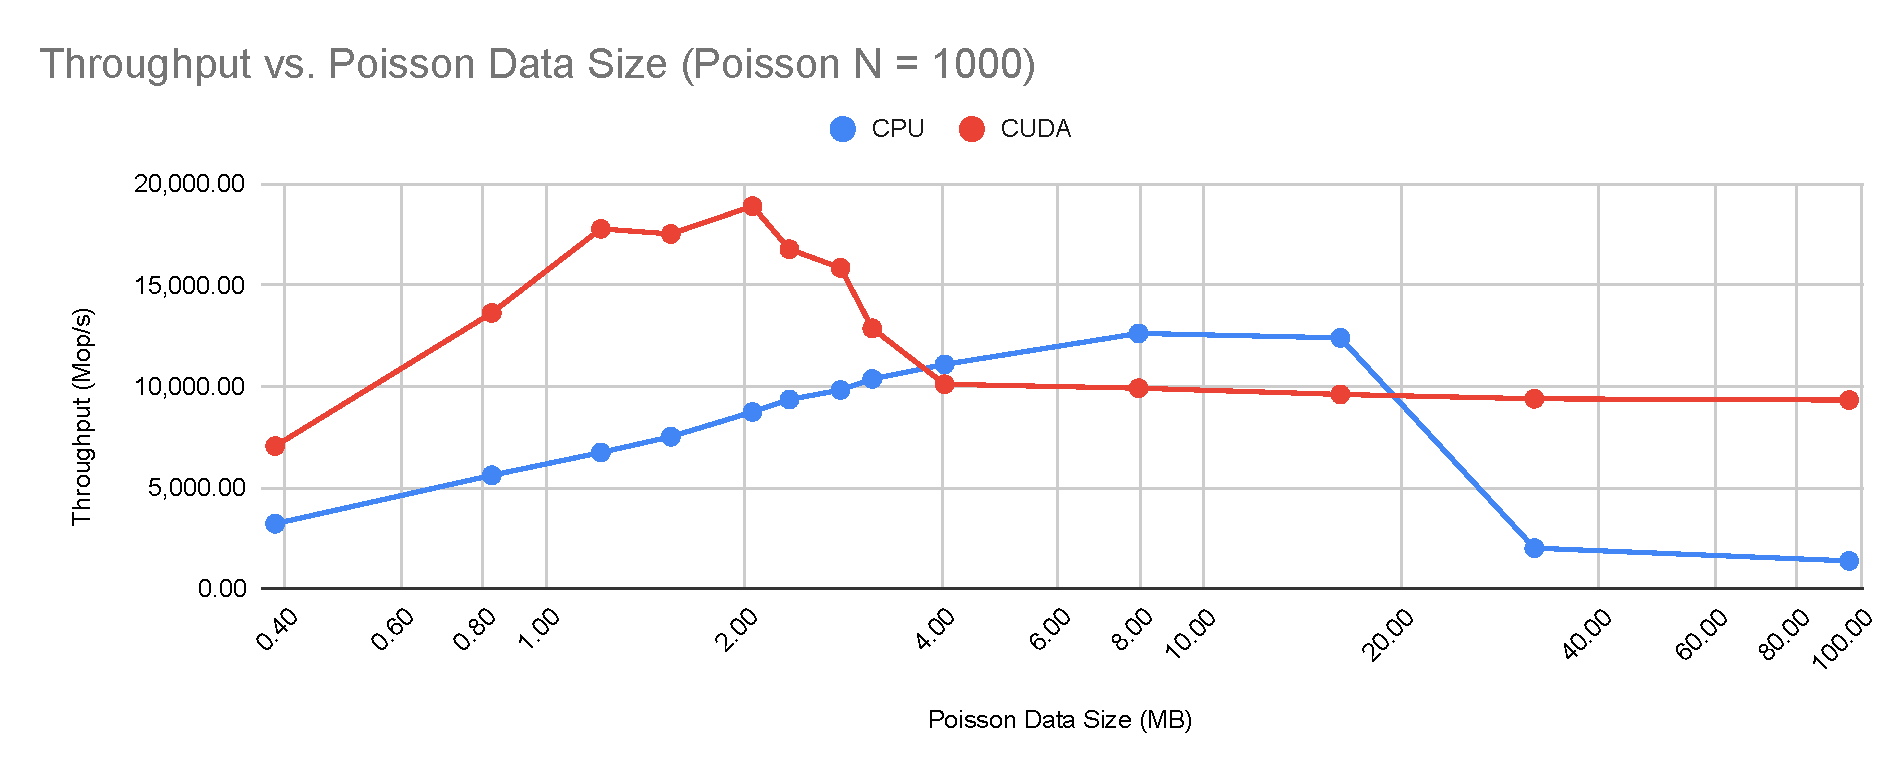
\includegraphics[width=\linewidth]{Ch62Results/figures/temp_throughput_over_size.pdf}
    \caption{Simulation Throughput for CPU and CUDA as required data size increases.}
    \label{fig:results:throughput_over_size}
\end{figure}

Initially, the biggest surprise in \cref{fig:results:throughput_over_size} was the CPU performing better than CUDA between 4-\SI{16}{\mega\byte}.
Other interesting points were the linear increase in CUDA throughput between 0.4-\SI{1.2}{\mega\byte}, and the performance plateau from \SI{4}{\mega\byte} onwards (CUDA) and \SI{32}{\mega\byte} onwards (CPU).
These are due to multiple factors, and are best explained by separating the CUDA graph into stages.
\todomark{Create a separate graph with each stage separated out?}
% (\todoref{figure with subfigures for each separate state}).

% \todoref{Throughput/Poisson - Inital climb state} shows \si{\mega\op\per\second} increasing almost linearly before plateauing at 1.2-\SI{1.5}{\mega\byte}.
The first stage shows \si{\mega\op\per\second} increasing almost linearly before plateauing at 1.2-\SI{1.5}{\mega\byte}.
This is due to the GPU's parallelization not being fully utilized.
This data was measured on a GTX 1080 which has 2560 CUDA cores separated into 20 Streaming Multiprocessors of 128 cores each\cite{nvidia1080Whitepaper}.
Each Multiprocessor can execute 2048~threads at once \todocite{https://docs.nvidia.com/cuda/cuda-occupancy-calculator/index.html}\todomark{(find better citation?)}, thus the GPU can execute at most 40,960~threads in parallel.
The first datapoint uses a 260~x~130 grid with only 33,800~cells, thus 16,900 threads per Poisson color stage\footnote{The red and black stages only write to the 1/2 of the grid corresponding to their color.}, so the GPU isn't saturated and isn't producing as many outputs as possible per second.
This is also the case for the second datapoint, with 36,100 threads per color stage.
Beyond this point, the GPU is saturated and the throughput plateaus.

\begin{table}[]
    \centering
    \begin{tabular}{c|ccc}
        Grid Size & Poisson Data Size (\si{\mega\byte}) & Total Cells & CUDA Threads per Color Stage \\
        \hline
        260x130 & 0.39 & 33,800 & 16,900 \\
        380x190 & 0.83 & 72,200 & 36,100 \\
        460x230 & 1.21 & 105,800 & 52,900 \\
        520x260 & 1.55 & 135,200 & 67,600 \\
        600x300 & 2.06 & 180,000 & 90,000 \\
        640x320 & 2.34 & 204,800 & 102,400 \\
        700x350 & 2.80 & 245,000 & 122,500 \\
        740x370 & 3.13 & 273,800 & 136,900 \\
        840x420 & 4.04 & 352,800 & 176,400 \\
        1180x590 & 7.97 & 696,200 & 348,100 \\
        1680x840 & 16.15 & 1,411,200 & 705,600 \\
        2360x1180 & 31.87 & 2,784,800 & 1,392,400 \\
        4096x2048 & 96.00 & 8,388,608 & 4,194,304 \\
    \end{tabular}
    \caption{Throughput Mesaurement Points}
    \label{tab:results:speeddata}
\end{table}

% The researcher believes is also the case for the second datapoint, a 380~x~190 grid with 72,200~cells, as the ramp-up time to fully saturate the GPU with threads (64 threads/mp / (32threads/warp * 2 warps/cycle) = 640 cycles) is significant compared to the time required to execute each thread.
% The decrease in \todoref{Throughput/Poisson - falling due to cache} begins after \SI{2}{\mega\byte}, which is the size of the GTX ~1080 L2 cache\cite{nvidia1080Whitepaper}.
The throughput decreases after \SI{2}{\mega\byte}, which is the size of the GTX~1080 L2 cache\cite{nvidia1080Whitepaper}.
As the size increases beyond this point the chances of a memory read being present in the cache decreases, so requests to main memory are made more frequently.
Main memory is much slower than L2 cache so the throughput decreases until the data is 2x the cache size (\SI{4}{\mega\byte}), at which point all accesses are to main memory and the throughput plateaus at \SI{10,000}{\mega\op\per\second}.
This behaviour can also be seen with the CPU, an AMD Ryzen 7 1800X with \SI{16}{\mega\byte} of L3 cache, which peaks at \SI{16}{\mega\byte} then drops at \SI{32}{\mega\byte} onwards.
Caching is vital to performance, and this program is no exception.
Adapting the implementation to better utilize cache is crucial to improving simulation speed at scale, and would be excellent to investigate this as future work.

\subsection{Accuracy}\label{sec:Results:Sim:Accuracy}
\newcolumntype{Z}{S[table-format=3.2]}
\begin{table}[ht]
    \centering
    \begin{tabular}{c|ZZZZ|ZZZZ}
        & \multicolumn{4}{c|}{Velocity} & \multicolumn{4}{c}{Pressure} \\
        \hline
        {Time (\si{\second})} & {100} & {200} & {300} & {1000} & {100} & {200} & {300} & {1000} \\
        \hline
        10 & -14.12 & -14.01 & -13.46 & -13.02 & -8.14 & -7.71 & -7.01 & -5.18 \\
        25 & -5.93 & -5.93 & -5.93 & -5.93 & -5.36 & -4.14 & -3.33 & -0.91 \\
        50 & -6.41 & -6.34 & -6.33 & -6.29 & -5.02 & -4.21 & -3.11 & -0.13 \\
    \end{tabular}
    \caption{Log of Mean Square Error between CPU and CUDA results\\(Numbers closer to 0 are worse)}
    \label{tab:results:accuracy_mse}
\end{table}
\begin{figure}
    \centering
    \subcaptionbox{Velocity MSE\label{fig:results:mse_velocity}%
    }[0.49\linewidth]{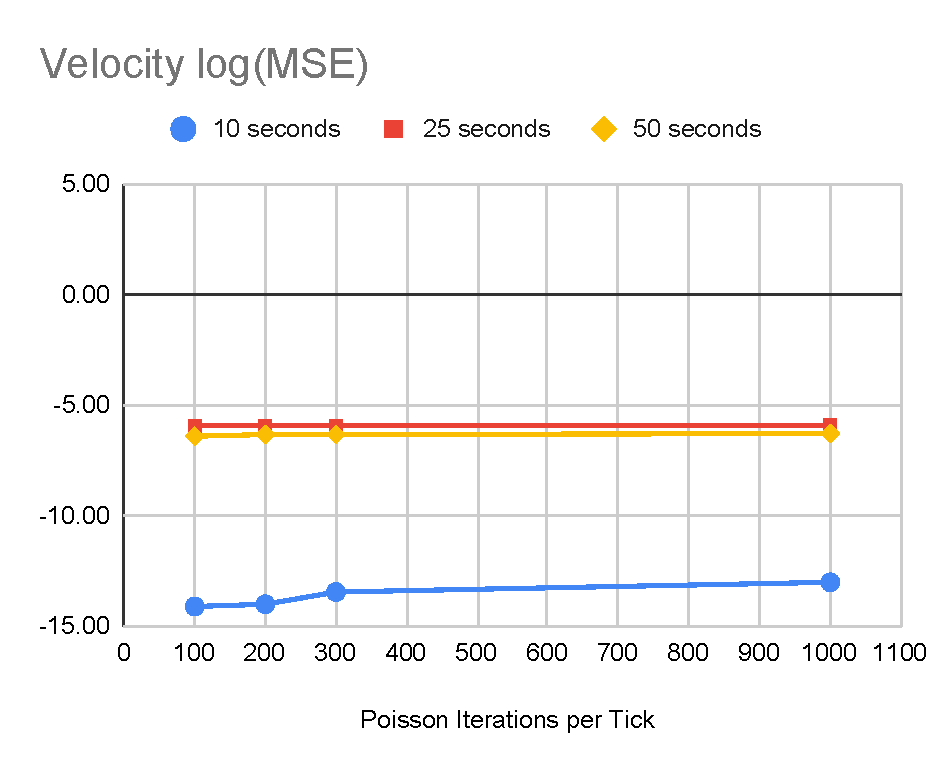
\includegraphics[width=\linewidth]{Ch62Results/figures/temp_velocity_mse.pdf}
    }%
    \subcaptionbox{Pressure MSE\label{fig:results:mse_pressure}%
    }[0.49\linewidth]{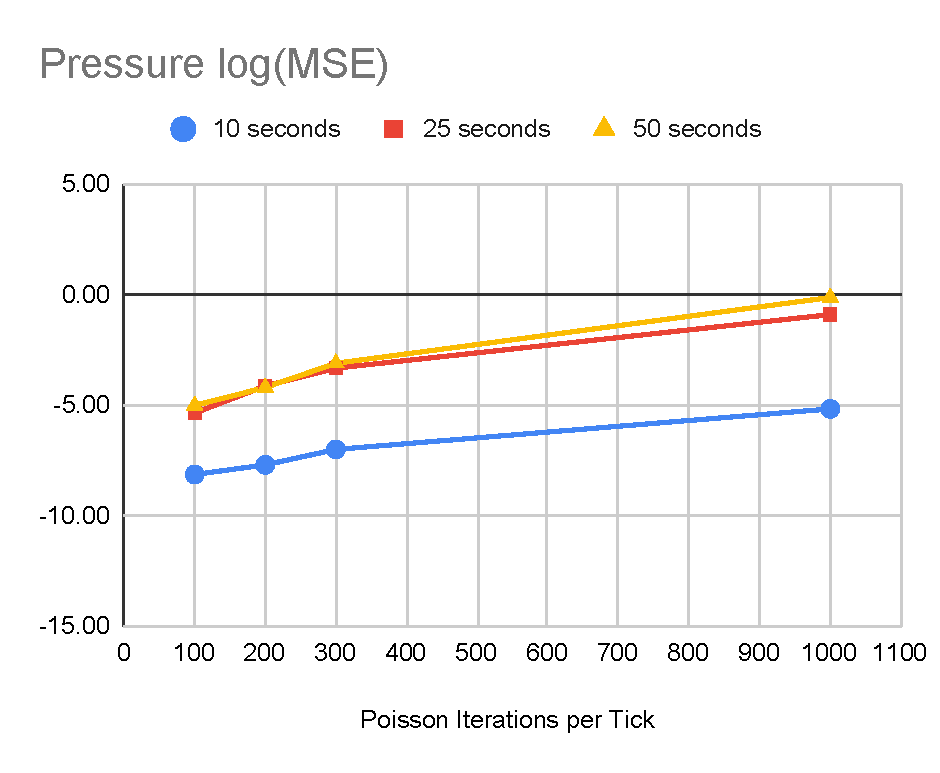
\includegraphics[width=\linewidth]{Ch62Results/figures/temp_pressure_mse.pdf}
    }    
    
    \caption{Initial MSE Results}
    \label{fig:results:mse_initial}
\end{figure}

Initially accuracy was measured by comparing the Mean Square Error between CPU and CUDA outputs after equivalent simulations (see \cref{tab:results:accuracy_mse}).
Ideally the CUDA and CPU results would be similar, and the MSE would be low (perhaps around $10^{-14}$, as expected in \cref{sec:Comparisons}.)
Instead the results are quite different - the velocity is quite similar after \SI{10}{\second}, but that delta increases to $10^{-6}$ as the simulation progresses.
Pressure is even worse, starting at $10^{-8}$ and going as far as a mean square error of $10^{0} = 1$.
In both cases the divergence between CPU and CUDA increases as more iterations are performed (see \cref{fig:results:mse_velocity,fig:results:mse_pressure}).
However, this isn't the whole story.
Measuring the difference between the CPU and CUDA doesn't show which one is more accurate.

\begin{table}[]
    \centering
    \begin{tabular}{c|S[table-format = 1.2e1]S[table-format = 1.2e1]|S[table-format = 1.2e1]c}
        Poisson Iterations & \multicolumn{1}{c}{Residual (CUDA)} &  \multicolumn{1}{c|}{Residual (CPU)} &  \multicolumn{1}{c}{Delta} &\\
        \hline
        100 & 6.34E-03 & 6.32E-03 & 1.88E-05 & (+0\%) \\
        200 & 1.49E-03 & 1.48E-03 & 1.73E-05 & (+1\%) \\
        300 & 6.49E-04 & 6.37E-04 & 1.16E-05 & (+2\%) \\
        1000 & 5.54E-05 & 5.28E-05 & 2.54E-06 & (+5\%) \\
        
    \end{tabular}
    \caption{Residual values after \SI{50}{\second} of simulation on original simulation input.}
    \label{tab:results:residual}
\end{table}

The true measure of accuracy for a differential equation solver is the precision of the solution - how close the values come to fulfilling the constraints of the equation.
The original simulation calculated this residual value as part of the Poisson loop, but this was removed for optimization purposes.
\cref{tab:results:residual} presents the residual values as calculated after the simulations completed, showing that the difference between CPU and CUDA in terms of the solver accuracy is very small.
CUDA is slightly less precise, but is at worst within just 5\% of the CPU residual.
This is likely forgivable for the sake of a real-time visualization, but could still be improved in the future.

% \begin{figure}
%     \centering
%     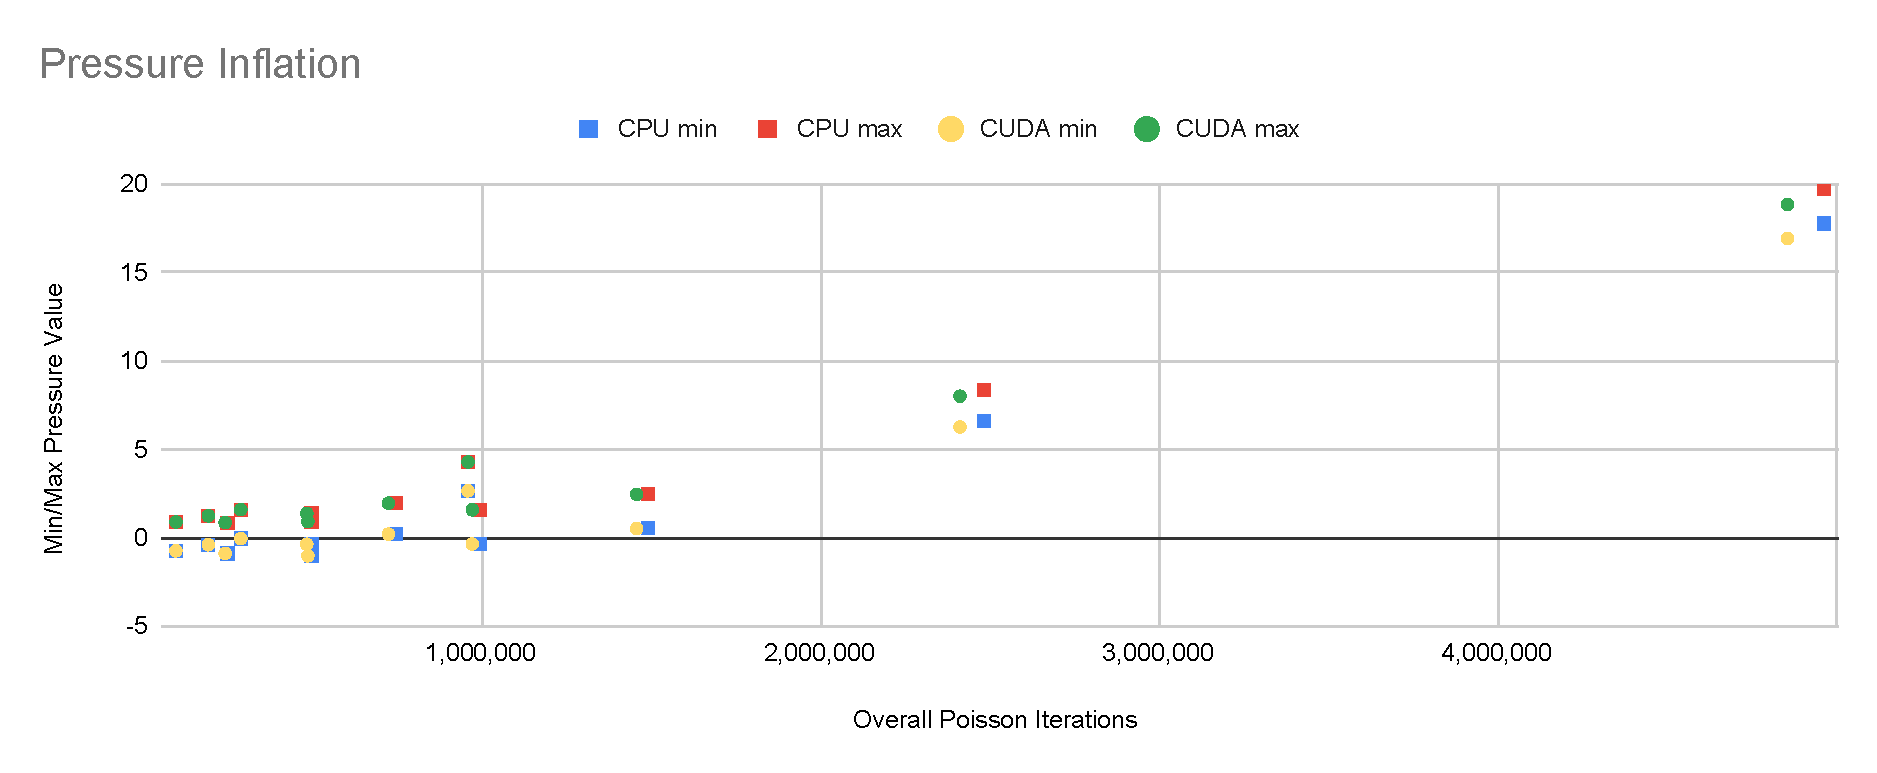
\includegraphics[width=\linewidth]{Ch62Results/figures/temp_pressure_inflation.pdf}
%     \caption{Inflation of pressure values with Poisson iterations}
%     \label{fig:results:pressure_inflation}
% \end{figure}

\begin{figure}
    \centering
    \begin{tikzpicture}
    \begin{axis}[
        title={Poisson Pressure Inflation},
        ylabel={Pressure Value Range},
        xlabel={Poisson Iterations},
        width=\linewidth,
        height=15em,
        ymin=-5, ymax=25,
        scaled x ticks = false,
        xtick={1000000, 2000000, 3000000, 4000000, 5000000},
        x tick label style={/pgf/number format/fixed},
        xmin=0, xmax=5000000,
        legend pos=north west
    ]
    \addplot+[only marks]%,draw=red] 
        plot [error bars/.cd, y dir=both, y explicit] 
        table [x=iters, y=cpu_mid, y error minus=delta_min_cpu, y error plus=delta_max_cpu, col sep=space, ignore chars={\,}] {Ch62Results/figures/data/pressure_inflation_cpu.csv};
    \addlegendentry{CPU};
    \addplot+[only marks]%,draw=blue] forget plot?
            plot [error bars/.cd, y dir=both, y explicit] 
            table [x=iters, y=cuda_mid, y error plus=delta_max_cuda, y error minus=delta_min_cuda, col sep=space, ignore chars={\,}] {Ch62Results/figures/data/pressure_inflation_cuda.csv};% 
    % \addplot table [x=cache, y=cuda, col sep=space, ignore chars={\,}] {Ch62Results/figures/data/pressure_inflation_cuda.csv};
    \addlegendentry{CUDA};

    \end{axis}
    \end{tikzpicture}
    \caption{Inflation of pressure values with Poisson iterations}
    \label{fig:results:pressure_inflation}
\end{figure}
% \begin{figure}
%     \centering
%     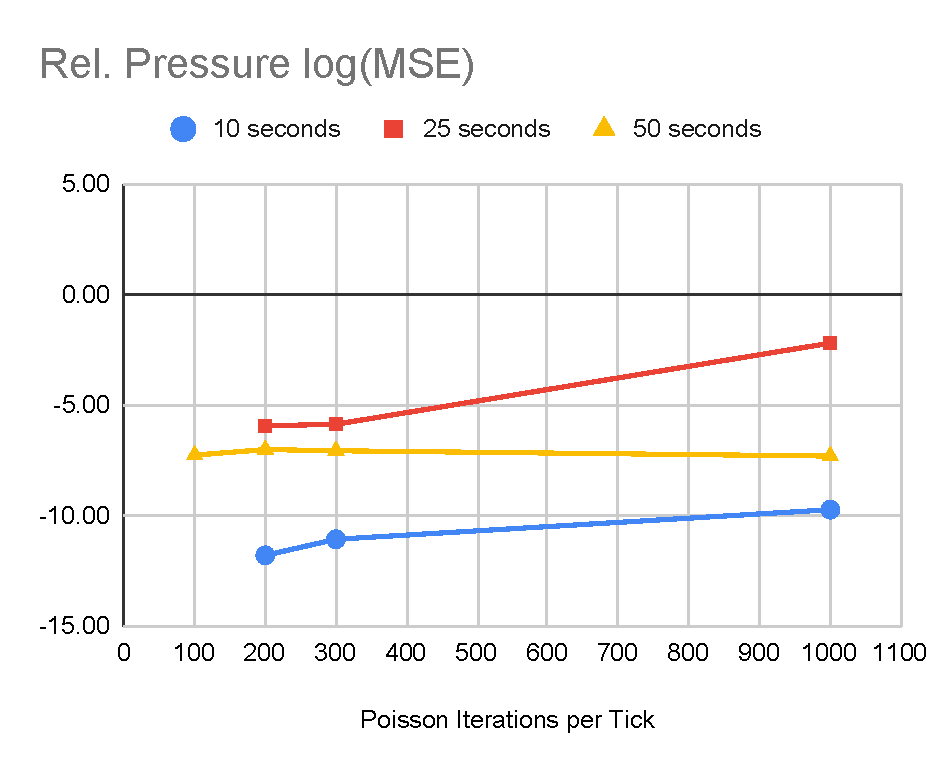
\includegraphics[width=0.5\linewidth]{Ch62Results/figures/temp_rel_pressure_mse.pdf}
%     \caption{MSE for Pressure when adjusted to use relative values}
%     \label{fig:results:mse_rel_pressure}
% \end{figure}

\begin{figure}
    \centering
    \begin{tikzpicture}
    \begin{axis}[
        title={Pressure (Relative) MSE},
        ylabel={MSE (log scale)},
        xlabel={Poisson Iterations per Tick},
        ymin=-15, ymax=5,
        xmin=0, xmax=1100,
        xtick={100,200,300,1000},
        ytick={5,0,-5,-10,-15},
        extra y ticks = {0},
        extra y tick labels = {},
        extra tick style = {
            grid=major,
            major grid style={line width=.5pt, draw=black}
        },
        yticklabels={$10^5$, $10^{0}$, $10^{-5}$, $10^{-10}$, $10^{-15}$},
        width=\linewidth,
        height=15em,
        legend pos = north east
    ]
    \addplot table [x=iters, y=pres-mean-10, col sep=space] {Ch62Results/figures/data/MSE.csv};
    % \addlegendentry{\SI{10}{\second}};
    \addplot table [x=iters, y=pres-mean-25, col sep=space] {Ch62Results/figures/data/MSE.csv};
    % \addlegendentry{\SI{25}{\second}};
    \addplot table [x=iters, y=pres-mean-50, col sep=space] {Ch62Results/figures/data/MSE.csv};
    % \addlegendentry{\SI{50}{\second}};
    \end{axis}
    \end{tikzpicture}
    \caption{MSE for Pressure when adjusted to use relative values}
    \label{fig:results:mse_rel_pressure}
\end{figure}




The large increase in Pressure MSE is explained by \cref{fig:results:pressure_inflation}.
The actual pressure values increase as more Poisson iterations are performed, for both CPU and CUDA.
CUDA's values inflate slightly more slowly, giving each grid cell a high square error, resulting in a large MSE.
When the MSE is calculated \emph{after} subtracting the mean from both datasets, i.e. comparing the relative values, the results are closer to the velocity MSE (\cref{fig:results:mse_rel_pressure}).
The pressure is only used internally as a relative value, so theoretically this inflation is fine, but in practice if it increases too much it could reach the limits of IEEE-754 floating point\cite{IEEEFloat75419} and cause accuracy/precision loss in the solver.
\cite{book:griebel1998numerical} mentioned that ``nonphysical pressure values'' may be the result of noncontinuous starting velocities, and mentioned a method for resolving this (see \cref{ext:PressureValues}). This may prevent the inflation, but it doesn't explain the deviation between the CPU and CUDA.

The CUDA and CPU compilers are configured to handle floating-point numbers slightly differently.
\texttt{nvcc} compiles with the \texttt{--fmad} option turned on by default\cite{NvccFmad} which ``enables the contraction of floating-point multiplies and adds/subtracts into floating-point multiply-add operations''.
This optimization performs a multiply and an addition at the same time, without a rounding step in between, resulting in a slightly more accurate result\cite{NvidiaFMAJustification}.
It is disabled for the CPU compiler, to keep the results from the other CPU backends consistent with the original ACA coursework.
While the change is subtle it's present in all CUDA kernels and when applied thousands of times may have a significant effect, leading to the deviation.
In the future this could be verified by compiling the CPU simulation with this option enabled.

\subsection{GPU Utilization}\label{sec:Results:Sim:Efficiency}
\begin{figure}
    \centering
    \begin{tikzpicture}
        \node[inner sep=0pt] (profile) at (0,0)
    {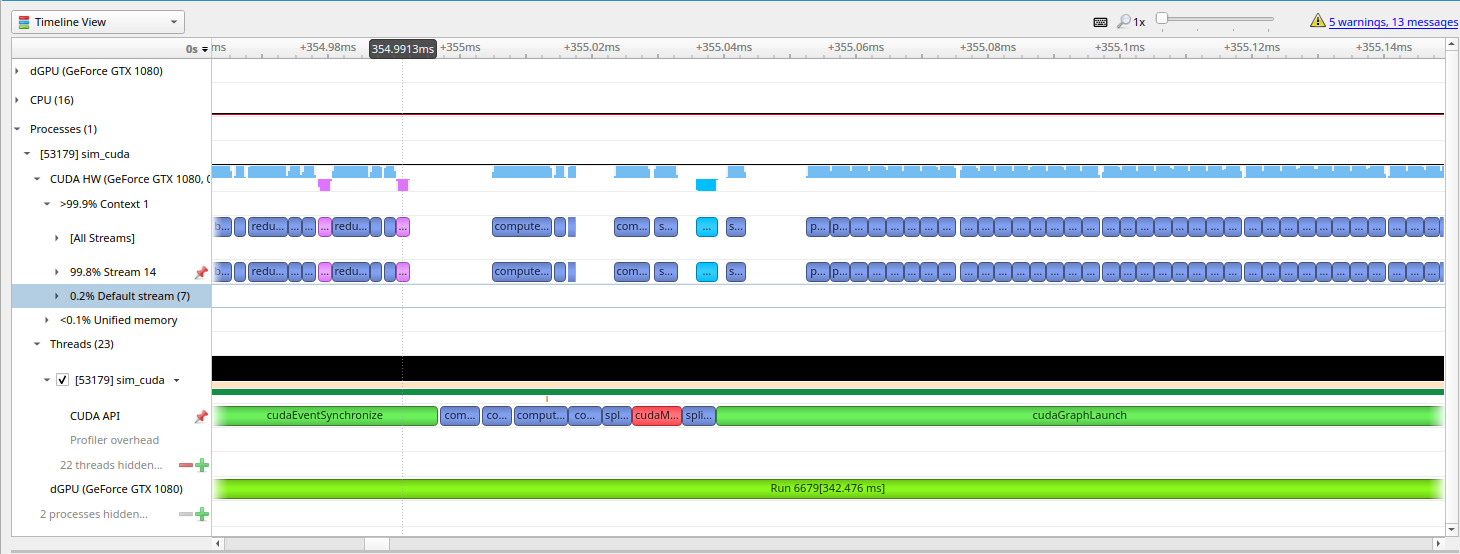
\includegraphics[width=1.0\linewidth]{Ch62Results/figures/temp_sim_profile.png}};
    
    \draw[line width=0.5mm] (-3.7, -0.1) -- ++(0, 2);% node[anchor=north east,align=right,fill=white] {GPU Reductions};
    \draw[line width=0.5mm] (-2.8, -0.1) -- ++(0,2);
    % \draw[line width=0.1mm] (-3.7, 1) -- (-2.8, 1);

    \draw[line width=0.5mm] (0.2, -0.1) -- ++(0, 2);
    \draw[line width=0.5mm] (0.9, -0.1) -- ++(0,2);
    
    % \draw[line width=0.1mm] (0.2, 1) -- (0.9, 1);
    
    \node[fill=white] at (-3.25, 1.9) {\SI{10}{\micro\second}};
    \node[fill=white] at (0.5, 1.9) {\SI{10}{\micro\second}};

    \end{tikzpicture}    
    \caption{Simulation Profile, highlighting the GPU bubbles}
    \label{fig:results:sim_profile_bubble}
\end{figure}
GPU Utilization is close to 100\% where possible.
During the Poisson iterations the GPU utilization is 100\% thanks to the CUDA Graph optimization.
At the tick boundaries, a bubble is unavoidable (see \cref{fig:results:sim_profile_bubble}) where the CPU has to wait for the GPU reductions to finish before calculating the timestep for the next tick and invoking the new calculations.
In practice this bubble is approximately \SI{10}{\micro\second} long, combined with another \SI{10}{\micro\second} long bubble between the Tentative Velocity stage finishing and the Poisson stage beginning.
Each tick at 100 iterations for the initial ACA took \SI{700}{\micro\second}, so this gap accounts for 2.8\% of the runtime.
As the simulation gets larger or the iteration count increases this gap should remain constant, and become even less significant.

\subsection{Memory Leaks}\label{sec:Results:Sim:Mem}
The program is designed to allocate all memory up-front, instead of allocating during a simulation.
This makes memory leaks unlikely, but not impossible.
\texttt{valgrind} was used to test if the program leaked any memory using the CPU backend.
Support for CUDA-based memory in \texttt{valgrind} seemed to be lacking, so it was run with suppressions enabled that hid CUDA-related false positives.
% \todocite{\url{https://forums.developer.nvidia.com/t/valgrind-3-4-suppressions-a-little-howto/7504}}
It did not find any leaks in the project code, but did find a potential memory leak in the OpenMP implementation\footnote{This may also be a false-positive similar to those from CUDA.}.
\texttt{cuda-memcheck} was then used to find any leaked CUDA memory, and found no potential leaks.
% \todomark{examples of results from both programs (check memory\_usage.tex)}

\section{Visualization}
\subsection{Speed}\label{sec:Results:Viz:Speed}
The speed of each individual feature was measured by enabling just that feature, moving to the worst-case for that feature such as enabling auto-range and maximizing onscreeen instances (\cref{tab:results:vizworstcases}), and then reading off the time-to-render from the GUI.
The rendered simulation state was the 660~x~120 ACA input, which is rendered internally at 2x resolution in both directions i.e. 1320~x~240 then composited with the GUI onto a 1600~x~900 window.

\begin{table}[]
    \centering
    \begin{tabular}{c|p{0.7\textwidth}}
        Feature & Worst-Case \\
        \hline
        Quantity-by-Scalar & Auto-range enabled \\
        Quantity-by-Vector & Auto-range enabled, grid spacing set to display maximum number of vectors = 10,000 \\
        Particle System & Particle simulation enabled, emitting maximum amount of particles per frame = 16, simulating and rendering maximum amount of particles = 100,000 \\
    \end{tabular}
    \caption{Testing Scenarios for Visualization Feature Speed.}
    \label{tab:results:vizworstcases}
\end{table}

\begin{table}
    \centering
    \begin{tabular}{|r|S[table-format=1.2,retain-explicit-plus]|S[table-format=1.2,retain-explicit-plus]|S[table-format=1.2,retain-explicit-plus]|S[table-format=1.2,retain-explicit-plus]|S[table-format=1.2,retain-explicit-plus]|}
    \hline
        & {Base Frame} & {with Sim} & {Scalar Quantity} & {Vector Field} & {Particles} \\ 
    \hline
        Mean Time (\si{\milli\second}) & 0.30 & 1.18 & 0.39 & 0.46 & 0.42 \\
        $\triangle$ from base (\si{\milli\second}) & {-} & +0.88 & +0.09 & +0.16 & +0.12 \\ 
    \hline
    \end{tabular}
    \caption{Visualization feature execution times}
    \label{tab:results:viz:speed}
\end{table}

The individual features are all faster than the simulation, even when combined, and are significantly shorter than the \SI{16.6}{\milli\second} required for a 60FPS visualization.
Even at scale, the visualization features should not have a significant impact on the visualization speed.

\subsection{GPU Utilization}\label{sec:Results:Viz:Efficiency}
\begin{figure}
    \centering
    \begin{tikzpicture}
        \node[inner sep=0pt] (profile) at (0,0)
    {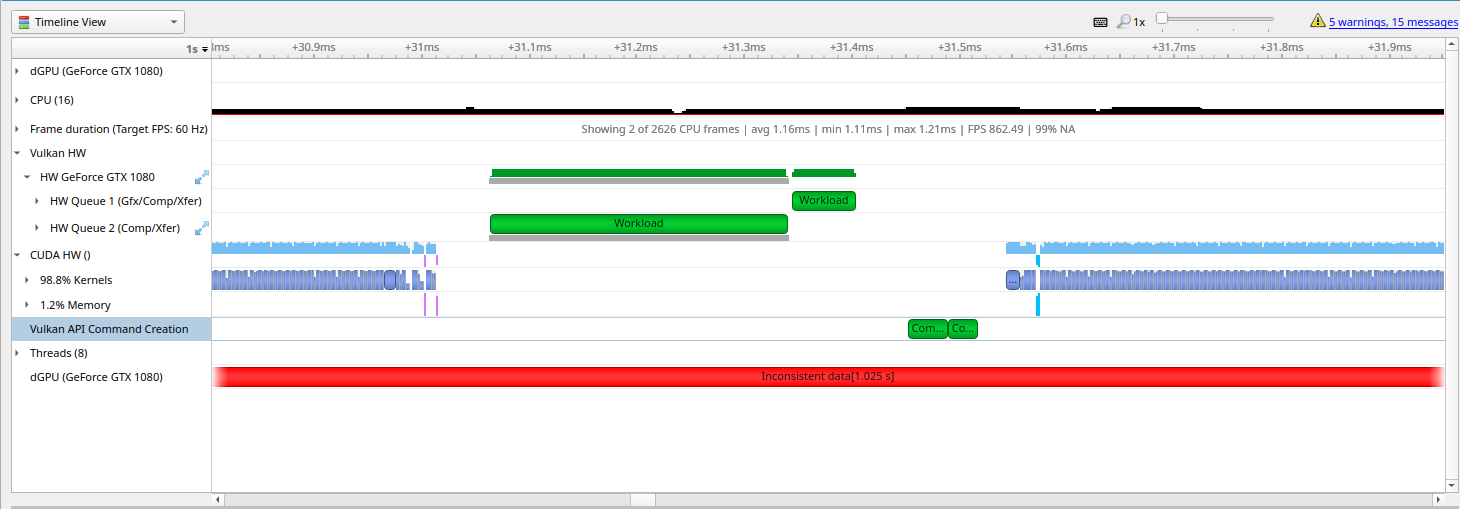
\includegraphics[width=1.0\linewidth]{Ch62Results/figures/temp_viz_profile.png}};
        
    \draw[line width=0.5mm,-Triangle] (-3.7, -0.5) -- ++(0, 1.8) -- ++(-0.21,0.0);% node[anchor=north east,align=right,fill=white] {GPU Reductions};
    % \draw[ultra thick,black,-Triangle] (vc.south west) -- (sim.north east) |- ++(0.25,0.5) ;
    \draw[line width=0.5mm] (-2.8, -0.5) -- ++(0,2);
    % \draw[line width=0.1mm] (-3.7, 1) -- (-2.8, 1);

    \draw[line width=0.5mm,-Triangle] (1.5, -0.5) -- ++(0, 1.8) -- ++(-0.21,0.0);
    \draw[line width=0.5mm] (3.2, -0.5) -- ++(0,2);
    
    % \draw[line width=0.1mm] (0.2, 1) -- (0.9, 1);
    
    \node[fill=white] at (-3.25, 1.8) {\SI{70}{\micro\second}};
    \node[fill=white] at (2.35, 1.8) {\SI{140}{\micro\second}};
    \end{tikzpicture}    
    \caption{Visualization Profile, highlighting the GPU bubbles}
    \label{fig:results:viz_profile_bubble}
\end{figure}
% the visualization work itself waits for around \SI{70}{\micro\second} before starting
%\todomark{This is time from semaphore, not time from reduction end, mark that on the graph}).

As for the Simulation, the GPU utilization is 100\% where possible.
Theoretically the visualization work would hide the extra latency from waiting for the reduction to finish, but in practice the visualization work itself waits for around \SI{70}{\micro\second} after the semaphore is raised before starting (\cref{fig:results:viz_profile_bubble}).
The next CUDA tick, which has been enqueued well in advance by the CPU, then takes \SI{140}{\micro\second} to start after the previous visualization rendering has finished.
In both cases there was no other GPU work executing for this program, or any other element of this program which could have delayed it, thus it must be due to outside factors e.g. the OS compositing system using the GPU to render the desktop.


\subsection{Memory Leaks}\label{sec:Results:Viz:Memory}
Testing the visualization for memory leaks proved more difficult than for the simulation.
Running \texttt{valgrind} with suppressions enabled found no errors in this program, but found many potential errors (or more likely false-positives) in the SDL2 windowing library and the underlying X windowing system.
\texttt{cuda-memcheck} produced a host of ``Invalid read'' errors, which seemed to originate from CUDA/Vulkan shared memory.
The documentation stated it could not handle DirectX interoperability\cite{NvidiaCudaMemcheckIssues}, but said nothing about Vulkan.
It suggested using the \texttt{compute-sanitizer} tool in other situations, which explicitly does not support Vulkan interoperability\cite{NvidiaComputeSanitizerRelease} and produced exactly the same errors.
Given that the errors were identical, it is very likely that both programs do not support Vulkan and should not be trusted.

As a last resort, the Memory Usage statistic from the Nvidia NSight Systems profiler was consulted.
This showed that the CUDA memory usage stayed constant, but had no option to show memory allocated in Vulkan.
As the Vulkan memory is all explicitly allocated at the start with smart resource manager classes it is incredibly unlikely that any Vulkan memory is leaked, but currently there are no tools able to verify this.